\documentclass[conference]{IEEEtran}
\usepackage{algorithmic}
\usepackage{amsmath,amssymb,amsfonts}
\usepackage{booktabs}
\usepackage{caption}
\usepackage{cite}
\usepackage{dirtree}
\usepackage{fancyhdr}
\usepackage[pdftex]{graphicx}
\usepackage{hyperref}
\usepackage{listings}
\usepackage{pgfplots}
\usepackage{pgfplotstable}
\usepackage{textcomp}
\usepackage{tikz}
\usepackage{url}
\usepackage{xcolor}
\usepackage{xspace}

\usetikzlibrary{positioning, arrows.meta}

\usetikzlibrary{pgfplots.groupplots}

\newcommand{\crayex}{HPE Cray EX\xspace} % standardize name for Cray EX platform
\newcommand{\craympich}{Cray-MPICH\xspace} % standardize name for cray mpich
\newcommand{\stackinator}{Stackinator\xspace} % standardize name the stackinator tool
\newcommand{\spack}{Spack\xspace} % standardize name for spack
\newcommand{\todo}[1]{\textbf{\textcolor{blue}{TODO: #1}}} % add a comment to the article
\newcommand{\assign}[1]{\textbf{\textcolor{blue!20!red}{TODO: #1}}} % add a comment to the article
\newcommand{\hilight}[1]{\textbf{\textcolor{blue!20!red}{#1}}} % add a comment to the article
\newcommand{\tocite}[1]{\textbf{\textcolor{blue!20!red}{[#1]}}} % mark missing citation
\newcommand{\sect}[1]{Section~\ref{#1}\xspace}  % consistent references to sections
\newcommand{\tbl}[1]{Table~\ref{#1}\xspace}  % consistent references to tables
\newcommand{\fig}[1]{Fig.~\ref{#1}\xspace}   % consistent references to figures
\newcommand{\eq}[1]{(\ref{#1})\xspace}   % consistent references to equations
\newcommand{\lst}[1]{\lstinline{#1}\xspace}   % shorthand for inline listing

\definecolor{codegreen}{rgb}{0,0.6,0}
\definecolor{codegray}{rgb}{0.5,0.5,0.5}
\definecolor{codepurple}{rgb}{0.58,0,0.82}
\definecolor{backcolour}{rgb}{0.95,0.95,0.95}

\lstdefinestyle{defaultstyle}{
    backgroundcolor=\color{backcolour},
    commentstyle=\color{codegreen},
    keywordstyle=\color{magenta},
    stringstyle=\color{codepurple},
    basicstyle=\ttfamily\footnotesize,
    breakatwhitespace=false,
    breaklines=true,
    captionpos=b,
    keepspaces=true,
    showspaces=false,
    showstringspaces=false,
    showtabs=false,
    tabsize=2
}

\lstset{style=defaultstyle}

\newcommand\YAMLcolonstyle{\ttfamily\color{magenta}\bfseries\footnotesize}
\newcommand\YAMLkeystyle{\ttfamily\color{blue!50!black}\bfseries\footnotesize}
\newcommand\YAMLvaluestyle{\ttfamily\color{green!50!black}\bfseries\footnotesize}

\makeatletter

% here is a macro expanding to the name of the language
% (handy if you decide to change it further down the road)
\newcommand\language@yaml{yaml}

\expandafter\expandafter\expandafter\lstdefinelanguage
\expandafter{\language@yaml}
{
  keywords={true,false,null,y,n},
  keywordstyle=\color{darkgray}\bfseries,
  basicstyle=\YAMLkeystyle,                                 % assuming a key comes first
  sensitive=false,
  comment=[l]{\#},
  morecomment=[s]{/*}{*/},
%  commentstyle=\color{purple}\ttfamily,
%  stringstyle=\YAMLvaluestyle\ttfamily,
  moredelim=[l][\color{orange}]{\&},
  moredelim=[l][\color{magenta}]{*},
  moredelim=**[il][\YAMLcolonstyle{:}\YAMLvaluestyle]{:},   % switch to value style at :
  morestring=[b]',
  morestring=[b]",
  literate =    {---}{{\ProcessThreeDashes}}3
                {>}{{\textcolor{red}\textgreater}}1     
                {|}{{\textcolor{red}\textbar}}1 
                {\ -\ }{{\mdseries\ -\ }}3,
}

% hyperlink formatting
\hypersetup{
    unicode=true,          % non-Latin characters in Acrobat’s bookmarks
    colorlinks=true,       % colored links
    linkcolor=blue,
    urlcolor=blue
}

\renewcommand\DTstyle{\footnotesize\tt}

\def\BibTeX{{\rm B\kern-.05em{\sc i\kern-.025em b}\kern-.08em
    T\kern-.1667em\lower.7ex\hbox{E}\kern-.125emX}}

\begin{document}

\title{Deploying Alternative User Environments on Alps}

\author{
\IEEEauthorblockN{Jonathan Coles}
    \IEEEauthorblockA{
        \textit{CSCS}\\
        Zurich, Switzerland \\
        jonathan.coles@cscs.ch
    }
\and
\IEEEauthorblockN{Ben Cumming}
    \IEEEauthorblockA{
        \textit{CSCS}\\
        Zurich, Switzerland \\
        bcumming@cscs.ch
    }
\and
\IEEEauthorblockN{Theofilos-Ioannis Manitaras}
    \IEEEauthorblockA{
        \textit{CSCS}\\
        Lugano, Switzerland \\
        theofilos.manitaras@cscs.ch
    }
\and
\IEEEauthorblockN{Jean-Guillaume Piccinali}
    \IEEEauthorblockA{
        \textit{CSCS}\\
        Lugano, Switzerland \\
        jgp@cscs.ch
    }
\and
\IEEEauthorblockN{Simon Pintarelli}
    \IEEEauthorblockA{
        \textit{CSCS}\\
        Zurich, Switzerland \\
        simon.pintarelli@cscs.ch
    }
\and
\IEEEauthorblockN{Harmen Stoppels}
    \IEEEauthorblockA{
        \textit{Stoppels Consulting/LLNL}\\
        Zurich, Switzerland \\
        harmen@stoppels.ch
    }
}

\maketitle

\begin{abstract}
We describe a method for defining, building and deploying alternative programming environments alongside the CPE on HPE Cray EX Alps infrastructure at CSCS.
This addresses an important strategic need at CSCS to deliver tailored environments within our versatile cluster (vCluster) configuration.
We provide compact, testable, optimized software environments that can be updated independently of the CPE release cycle.
The environments are defined with a descriptive YAML recipe, which is processed by a novel configuration tool that builds the software stack using Spack and generates a SquashFS image.
\craympich is provided through a custom Spack package without the need for a CPE installation.
We describe the command line tools and Slurm plugin that facilitate loading environments per user and per job.
Through a series of benchmarks we demonstrate application and micro-benchmark performance that matches CPE.

%%% Local Variables:
%%% TeX-master: "paper"
%%% End:

\end{abstract}

\begin{IEEEkeywords}
CPE, squashfs, slurm, spack
\end{IEEEkeywords}

\section{Introduction}
CSCS is deploying logically isolated, versatile software-defined clusters (vClusters)\cite{vClusters2023} on the \crayex system Alps, to provide services to a wider range of user domains, each with their own software, security, reliability and scaling requirements.
The vClusters can be customized for each target use case, as an alternative to one large system that offers a ``one size fits all'' programming environment, storage and job scheduler configuration.

CSCS aims to reduce the complexity of the software installed on each vCluster through tailored user environments (uenv's).
These environments will provide the smallest possible set of compilers, libraries and tools optimized for vCluster's requirements, node architecture and the Slingshot 11 interconnect.
One obvious use case is for single purpose clusters, e.g., the production cluster of the Swiss weather service.
Alternatively, multiple use-case specific environments can be provided on general-purpose HPC vClusters, and loaded according to a user's individual needs.

This approach is at odds with the widely-adopted method to provide software on \crayex systems: installing the Cray Programming Environment (CPE), and building use-case specific software not provided by CPE on a shared file system, as illustrated in~\fig{fig:stacks}(a).
The CPE provides a wide range of software -- compilers, scientific libraries, communication libraries, debuggers, profiling tools, etc. -- all optimised for the node and network architecture of the system.
Furthemore, Cray continues to evolve and expand the CPE in response to changing requirements, for example adding software packages for ML/AI, with quarterly releases to address bugs, improve performance and add features.
Indeed, CSCS currently delivers such a one-size-fits-all environment, similarly to other HPC sites, using EasyBuild to provide additional software built and maintained by CSCS~\cite{forai:cug16}.

\begin{figure*}[htp!]
    \begin{center}
        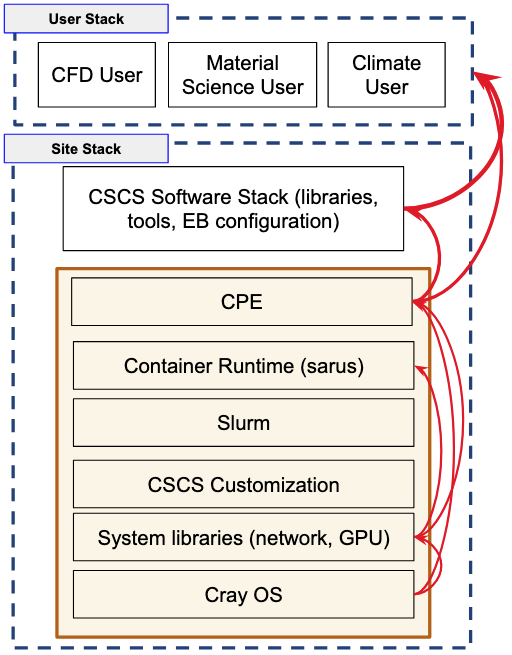
\includegraphics[width=0.35\textwidth]{./images/stack-old.png}
        \hspace{2.5cm}
        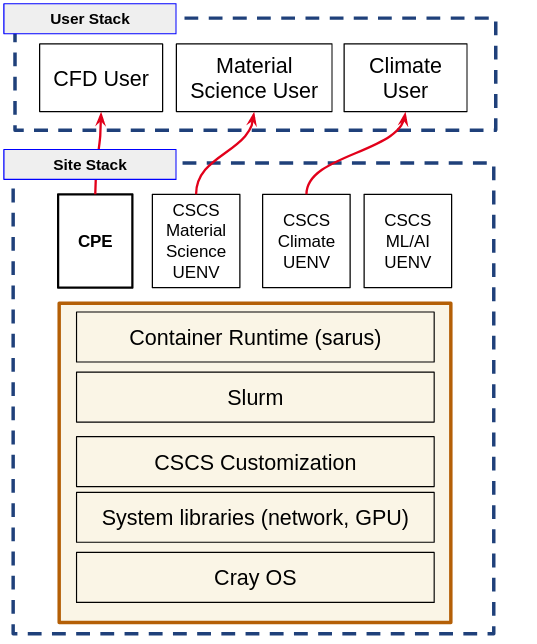
\includegraphics[width=0.35\textwidth]{./images/stack-new.png}
        \\
        \textbf{(a)} \hspace{9cm} \textbf{(b)}\\
    \end{center}
    \caption{
        \textbf{(a)}:
        The ``standard'' HPE-EX software stack, with the Cray OS, drivers, CPE and site-specific software in the system image, site-provided software installed on a shared file system. 
        User-installed software depends on the software layers underneath.
        The red arrows indicate where changes to one layer have a knock on effect on other software layers, requiring rebuilds or reconfiguration.\newline
        \textbf{(b)}:
        The Alps software stack with the programming environment moved out of the base image.
        Multiple programming environments can be deployed on top of this architecture. The CPE, and alternative PEs discussed in~\sect{sec:spack-stacks}, are mounted at runtime in a new mount namespace by users.
    }
    \label{fig:stacks}
\end{figure*}

However, while the CPE is a good general purpose environment for users, using it as a layer in HPC software stacks conflicts with our aim of reducing the complexity of software stacks.
In particular, two issues arise:
\begin{itemize}
    \item No single use-case or domain will use more than a small subset of the features provided by the CPE;
    \item Due to the CPE's quarterly cycle, the lead time between identifying an issue and a fix available and tested on site can be expected to be in the order of 3-6 months;
\end{itemize}
By striking a balance between long term stability and providing up-to-date software versions, CPE cannot fully satisfy use cases that only require either stability or timely fixes.

The work presented in this paper uses \spack and SquashFS images to build and deploy software stacks on top of a simplified base image that provides only the necessary vendor-specific libraries, for example libfabric, as illustrated in \fig{fig:stacks}(b).
Such a base image changes less frequently than CPE, reducing the need to rebuild software stacks with each CPE update and reducing system dependencies that could require intervention.

The result is compact, testable, reproducible and optimized software environments based on a descriptive recipe that can be updated independently of the CPE release cycle.

%\begin{enumerate}
%    \item long term stability -- software stack configuration can be maintained for longer
%    \begin{itemize}
%        \item requirement: reproducible builds
%        \item requirement: concise descriptive  recipes
%        \item requirement: minimise system requirements to only the bare minimum (no CPE)
%    \end{itemize}
%    \item rolling releases and fast fixes -- be able to rebuild and reconfigure at any point
%    \item provide use-case or application specific environments (only provide the required minimum)
%    \begin{itemize}
%        \item requirement: versioning of environments
%        \item requirement: fast deployment
%    \end{itemize}
%    \item deliver a satisfying user experience
%    \begin{itemize}
%        \item building and configuring software is fast and consistent (not dependent on file system performance).
%        \item compatibility with module, spack, python venv workflows.
%    \end{itemize}
%\end{enumerate}


%%% Local Variables:
%%% TeX-master: "paper"
%%% End:


\section{Spack Stacks}
\label{sec:spack-stacks}
\assign{Ben}

todo{missing points}
\begin{itemize}
    \item bubblwrap to mount the build path at the mount point to during build steps so that images can be built at locations for which the does not have write permissions.
    \item the tooling can generate spack-stacks that can be deployed as squashfs images, or on a shared file system.
    \item store is the location of the stack, with the compiled packages, a spack upstream configuration, optional module files and. The contents can either be copied to the target mount point, or compressed in a squashfs image that can be mounted on demand by users.
    \item introduce the nvidia PE that we use as an example.
\end{itemize}

We present a workflow and tooling for building separate PE stacks, tailored for use-cases, on top of the simplest possible base node image, that is built on CrayOS and core dependencies such as libfabric and rdma-core, without CPE installed.

The main tool is \href{https://github.com/eth-cscs/stackinator}{\stackinator}, which uses \spack~\cite{gamblin:sc15} to build complete PEs in a directory, which can then be deployed as squashfs images or as directories on a shared file systembuild complete PEs in a directory, which can then be deployed as squashfs images or as directories on a shared file system.

\stackinator is an open-source Python application, that makes is \emph{opinionated}\footnote{minimal changes are required to generate stacks for other systems -- a version that generates stacks for AWS Gravitron 3 clusters was created in a hackathon.}, in the sense that it:
\begin{itemize}
    \item reduces the complexity of specifying PEs that require reproducable 
    \item Makes design decisions that focus on reproducability and performance tuning for the target SlingShot 11 network and node-architectures available on Alps.
    \item provides limited configuration options for compilers -- the tool configures the full compiler spec according to CSCS best practices.
    \item provides limited configuration options for MPI -- only cray-mpich is supported fully, and in the future MPICH and OpenMPI will be supported, for which the tool will configure for Slingshot 11 and accelerator compatibility.
\end{itemize}

The following sections describe the workflow, from recipe to squashfs-images, and the novel and \crayex-specific implementation details.

%%%%%%%%%%%%%%%%%%%%%%%%%%%%%%%%%%%%%%%%%%%%%%%%
\subsection{Stack Specification}
%%%%%%%%%%%%%%%%%%%%%%%%%%%%%%%%%%%%%%%%%%%%%%%%

The discussion of the spack recipes motivated will be motivated by an example stack for development on nodes with NVIDIA A100 GPUs:
\begin{itemize}
    \item A GCC 11.3 compiler tool chain.
    \item An NVHPC 22.7 compiler tool chain.
    \item A GCC programming environment "gcc-env" with CUDA-aware cray-mpich, OSU Benchmarks, OpenBlas and CUDA 11.8.
    \item An NVHPC programming environment "openac-env" with CUDA-aware cray-mpich, OSU Benchmarks and CUDA 11.8.
\end{itemize}

Spack stacks are generated from a descriptive YAML file recipe, composed of the following:
\begin{itemize}
    \item  \lstinline{config.yaml}:
        \lstinputlisting[language=yaml]{src/nv-recipe/config.yaml}
        Used to specify where the image will be installed/mounted (the CSCS default is \emph{/user-environment}), optional configuration for a \spack build cache and the version of spack. Reproducable builds use a fixed version/commit of \spack, and rolling releases use the \lst{develop} branch of \spack.
    \item \lstinline{compilers.yaml} describes the compiler toolchains:
        \lstinputlisting[language=yaml]{src/nv-recipe/compilers.yaml}
        The bootstrap and GCC toolchains are mandatory, and it is allowed to specify more than one version of GCC.
        The llvm toolchain is optional, with support for installing multiple versions of the NVIDIA HPC-SDK and llvm/Clang.
    \item \lst{environment.yaml} describes the software packages;
        \lstinputlisting[language=yaml]{src/nv-recipe/environments.yaml}
        The software packages are configured as environments, each with built using the compiler toolchaines built previously, and configured with a (optional) single implementation of cray-mpich, that can optionally be configured for CUDA or ROCM support.
    \item \lst{packages.yaml} and \lst{modules.yaml}
        for making \spack use packages installed on the system, and generating modules files respetively.
        These follow the YAML specifications for the \spack configuration files with the same names.
    \item \lst{repo}
        is an optional path containing a \href{https://spack.readthedocs.io/en/latest/repositories.html}{\spack repository}, for overriding \spack's implementations or providing support for new packages.
\end{itemize}

Under the hood, the software in the stack is built in a set of \spack environments.
For the example stack there are five environments, illustrated in~\fig{fig:env-dag}.

\begin{figure}[htp!]
    \begin{center}
    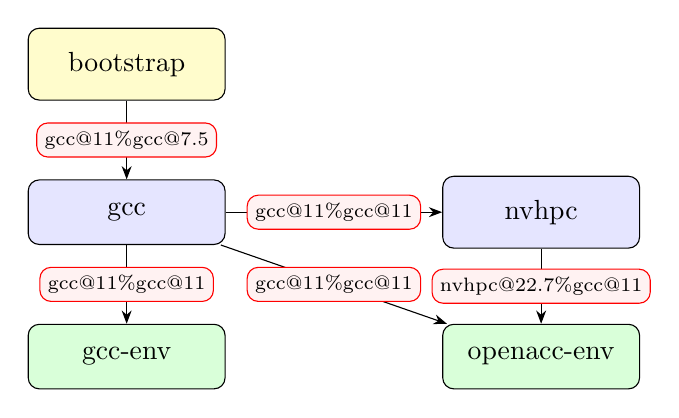
\begin{tikzpicture}[node distance=1cm and 2.75cm,
            nodes={draw, rectangle, rounded corners, minimum height=0.5cm, minimum width=2.5cm, fill=blue!10, inner sep=0.3cm},
            arrows={-Stealth}]
    % Nodes
    \node[fill=yellow!20] (bootstrap) {bootstrap};
    \node[below=of bootstrap] (gcc) {gcc};
    \node[right=of gcc] (nvhpc) {nvhpc};
    \node[fill=green!15, below=of gcc] (gcc-env) {gcc-env};
    \node[fill=green!15, right=of gcc-env] (openacc-env) {openacc-env};

    % Edges
    \draw (bootstrap)
        edge node[midway, fill=white,rectangle,fill=red!5, draw=red, inner sep=0.1cm, minimum height=0.3cm, minimum width=1 cm]
        {\scriptsize gcc@11\%gcc@7.5}
        (gcc);
    \draw (gcc) 
        edge node[midway, fill=white,rectangle,fill=red!5, draw=red, inner sep=0.1cm, minimum height=0.3cm, minimum width=1 cm]
        {\scriptsize gcc@11\%gcc@11}
        (nvhpc);
    \draw (gcc) 
        edge node[midway, fill=white,rectangle,fill=red!5, draw=red, inner sep=0.1cm, minimum height=0.3cm, minimum width=1 cm]
        {\scriptsize gcc@11\%gcc@11}
        (gcc-env);
    \draw (gcc) 
        edge node[midway, fill=white,rectangle,fill=red!5, draw=red, inner sep=0.1cm, minimum height=0.3cm, minimum width=1 cm]
        {\scriptsize gcc@11\%gcc@11}
        (openacc-env);
    \draw (nvhpc) 
        edge node[midway, fill=white,rectangle,fill=red!5, draw=red, inner sep=0.1cm, minimum height=0.3cm, minimum width=1 cm]
        {\scriptsize nvhpc@22.7\%gcc@11}
        (openacc-env);
\end{tikzpicture}

    \end{center}
    \caption{The dependency graph between the spack environments that are built to provide a spack stack that provides gcc 11 and nvhpc 22.7 toolchains, and two environments built with the compilers. The bootstrap compiler is built first using the system gcc 7.5. Then gcc 11 toolchain, followed by the nvhpc toolchain which requires gcc 11. Finally two environments are built: gcc-env with gcc 11, and openacc-env which contains pacakges built with both gcc 11 and nvhpc 22.7.}
    \label{fig:env-dag}
\end{figure}

The spack stack requires external packages installed on the base node image, that implement architecture-specific features and support, and can vary between vClusters and over time.
For example, the location of libfabric moves every time the installed version of libfabric is upgraded. 
A set of ``cluster configurations'' for each of the vClusters on Alps is maintained separately from the recipes in the \stackinator tool:
\begin{itemize}
    \item A \spack \lst{compilers.yaml} file that specifies the default GCC compiler toolchain on the vCluster (GCC 7.5 at the time of writing), used to bootstrap the spack stack build.
    \item A \spack \lst{packages.yaml} file that specifies externally installed software packages that Spack should never build, including:
    \begin{itemize}
        \item \lst{libfabric}: the libfabric library installed in \lst{/opt/cray/libfabric/} with CXI provider.
        \item \lst{slurm}: VClusters can have different versions of SLURM installed: at the time of writing versions 20.11.9 and 22.05.2 are used.
        \item \lst{xpmemm} and \lst{rdma-core}: required by some communication libraries.
    \end{itemize}
\end{itemize}

%%%%%%%%%%%%%%%%%%%%%%%%%%%%%%%%%%%%%%%%%%%%%%%%
\subsection{Stack Configuration and Building}
%%%%%%%%%%%%%%%%%%%%%%%%%%%%%%%%%%%%%%%%%%%%%%%%

\stackinator follows the familiar configure-build-install workflow used to install software.
It provides a CLI tool \lstinline{stack-config}, that takes a generic recipe that can be built on any (vCluster, mount point) combination, and generates a build path that contains a Makefile, \spack environment descriptions, and a copy of \spack used to build the stack.

If the recipe that describes the example environment in~\fig{fig:env-dag} is in the path \lstinline{~/recipes/nvidia}, \lstinline{stack-config} can be used to generated a build configuration with the following command:
\begin{lstlisting}
> stack-config -r ~/recipes/nvidia \
             -b /dev/shm/nvidia-build \
             -s hohgant \
\end{lstlisting}
where the generated build path is in \lstinline{/dev/shm/nvidia-build} and the build is configured for the vCluster Hohgant.
A simplified version of the build directory structure is illustrated in~\fig{fig:build-tree}.

\begin{figure}[htp!]
    \dirtree{%
.1 /dev/shm/nvidia-build.
.2 Makefile.
.2 spack.
.2 compilers.
.3 Makefile.
.3 bootstrap.
.4 spack.yaml.
.4 \textcolor{blue}{compilers.yaml}.
.4 \textcolor{blue}{packages.yaml}.
.4 \textcolor{blue}{Makefile}.
.3 gcc.
.4 spack.yaml.
.3 llvm.
.4 spack.yaml.
.2 environments.
.3 Makefile.
.3 gcc-env.
.4 spack.yaml.
.3 nvhpc-env.
.4 spack.yaml.
.2 store.
}


    \caption{Structure of the build path generated by the \stackinator tool. The files marked in blue are generated by calls to \spack during the build process in each of the five environment paths, and are only shown in the boostrap path for brevity.}
    \label{fig:build-tree}
\end{figure}

The environment is built using the top-level Makefile, which executes the following steps:
\begin{enumerate}
    \item configure build cache (*)
    \item (*) configure build cache
    \item call \lst{compilers/Makefile}:
    \begin{enumerate}
        \item concretise bootstrap
        \item build bootstrap
        \item concretise gcc
        \item build gcc
        \item concretise llvm (nvhpc)
        \item build llvm (nvhpc)
    \end{enumerate}
    \item call \lst{environments/Makefile}:
    \begin{enumerate}
        \item concretise gcc-env and nvhpc-env concurrently
        \item build gcc-env and nvhpc-env concurrently
    \end{enumerate}
    \item generate \lst{store/config}
    \item (*) generate \lst{store/modules}
    \item generate squashfs image of \lst{store}
\end{enumerate}


The \lstinline{compilers.yaml}, \lstinline{packages.yaml} and \lstinline{Makefile} for each of the spack environments are generated in the Makefile using spack. The commands used generate the respective files required to build the "gcc-env" are summarised:
\begin{itemize}
    \item \lst{gcc-env/compilers.yaml}:
        \begin{lstlisting}
> gcc_prefix= spack -e ../compilers/gcc \
        find --format '{prefix}' gcc@11
> spack compiler find --scope=user \
        $(compiler_bin_dirs $gcc_prefix)
        \end{lstlisting}
        Where the function \lst{compiler_bin_dirs} is a function that returns \lst{bin} path of the compiler, omitted for brevity.

    \item \lst{gcc-env/packages.yaml}:
        \begin{lstlisting}
> spack external find --not-buildable --scope=user  perl diffutils gettext
        \end{lstlisting}

    \item \lst{gcc-env/Makefile}:
        \begin{lstlisting}
        > spack -e gcc-env/ concretize -f
        > spack -e gcc-env/ env depfile -o gcc-env/Makefile
        \end{lstlisting}
        First, the environment is concretized (\spack generates the full set of packages and their dependencies for the environment), then a Makefile that facilitates building packages in parallel is generated.
\end{itemize}

\begin{lstlisting}
> cd /dev/shm/nvidia-build
> env --ignore-environment \
    PATH=/usr/bin:/bin:`pwd`/spack/bin \
    make store.squashfs -j32
\end{lstlisting}
The \lst{env} command is used to improve reproducability by eliminating the effect of environment variables on the build.

%%%%%%%%%%%%%%%%%%%%%%%%%%%%%%%%%%%%%%%%%%%%%%%%
\subsection{MPI}
%%%%%%%%%%%%%%%%%%%%%%%%%%%%%%%%%%%%%%%%%%%%%%%%
Open source MPI distributions -- namely OpenMPI, MVAPICH3 and MPICH -- are actively developing support for Slingshot 11 with libfabric.
However, at the time of writing the only MPI with robust Slingshot 11 support is the \craympich bundled with the CPE, for which source code is not available.

One of the objectives of this work is to provide software stacks without installing CPE.
In order to provide \craympich, we develop a process for repackaging the compiler wrappers, library, headers and dependencies like PMI that can be installed as a spack binary package.

%%%%%%%%%%%%%%%%%%%%%%%%%%%%%%%%%%%%%%%%%%%%%%%%
\noindent\textbf{Step 1: extract and repackage RPMs}
%%%%%%%%%%%%%%%%%%%%%%%%%%%%%%%%%%%%%%%%%%%%%%%%

Expand the following RPMs from the CPE distribution:
\begin{enumerate}
    \item \lst{cray-mpich-8.1.18-gnu91-0-4.sles15sp3.x86_64.rpm}
    \begin{itemize}
        \item The \
        \item For the NVIDIA HPC SDK use \lst{cray-mpich-8.1.18-nvidia207-0-4.sles15sp3.x86_64.rpm}.
    \end{itemize}
    \item \lst{cray-mpich-8.1.18-gtl-0-4.sles15sp3.x86_64.rpm}
    \begin{itemize}
        \item The GTL (GPU Transport Layer) libraries that implement GPU-aware communication for NVIDA and AMD GPUs.
    \end{itemize}
    \item \lst{cray-pmi-[version].rpm}
\end{enumerate}

We can't provide a single binary distribution for all compilers, because the Fortran modules in the \lst{include} path are compiler specific.

Extract headers, binaries and libraries from the RPMs, and gather them in a directory with structure illustrated in~\fig{fig:mpich-tree}.

\begin{figure}[htp!]
    \input{src/cray-mpich-tree-nosym.txt}
    \caption{ Note that for brevity symlinked library files are removed, and wildcards are used to describe headers.}
    \label{fig:mpich-tree}
\end{figure}


%%%%%%%%%%%%%%%%%%%%%%%%%%%%%%%%%%%%%%%%%%%%%%%%
\noindent\textbf{Step 2: patch MPI wrappers}
%%%%%%%%%%%%%%%%%%%%%%%%%%%%%%%%%%%%%%%%%%%%%%%%

As opposed to the CPE, which provides the \lst{CC}, \lst{cc} and \lst{ftn} binary compiler wrappers, our package uses the MPI compiler wrapper scripts that are installed in locations like \lst{/opt/cray/pe/mpich/8.1.21/ofi/gnu/9.1/bin}.

By default, these wrappers use environment variables set by CPE modules to select the compiler and link architecture-specific libraries.
Each of the wrappers is parameterised on three parameters \lst{@CC@}, \lst{@@PREFIX@@} and \lst{@@GTL_LIBRARY@@}, which are later set by spack to:
\begin{itemize}
    \item hard code the full path to the wrapped compiler;
    \item set paths \lst{prefix}, \lst{includedir}, to the cray-mpich \spack installation path;
    \item explicitly link \lst{-lmpi_gtl_cuda} \lst{-lmpi_gtl_hsa} when \craympich is built with the \lst{+cuda} or \lst{+rocm} variants respectively.
    \begin{itemize}
        %\item this fixes the common runtime error ``MPIDI\_CRAY\_init: GPU\_SUPPORT\_ENABLED'' is requested, but GTL library is not linked.
        \item hello world
    \end{itemize}
\end{itemize}


%%%%%%%%%%%%%%%%%%%%%%%%%%%%%%%%%%%%%%%%%%%%%%%%
\noindent\textbf{Step 3: create patch binary spack package}
%%%%%%%%%%%%%%%%%%%%%%%%%%%%%%%%%%%%%%%%%%%%%%%%

The 
The tar balls are stored in a \href{https://jfrog.com/artifactory/}{JFrog Artifactory} -- a self-hosted artifact store accessible only on the CSCS network.
The \spack package directly downloads from the artifactory, so it can only be run on CSCS systems.

\href{https://github.com/eth-cscs/stackinator/blob/master/stackinator/repo/packages/cray-mpich/package.py}{\lst{/stackinator/repo/packages/cray-mpich/package.py}}

%%%%%%%%%%%%%%%%%%%%%%%%%%%%%%%%%%%%%%%%%%%%%%%%
\subsection{Efficient Stack Builds}
%%%%%%%%%%%%%%%%%%%%%%%%%%%%%%%%%%%%%%%%%%%%%%%%

Using Spack to build a full software stack -- with multiple compilers, libraries and tools -- is time and resource consuming.
A simple stack based on GCC that provides Python, \craympich and cuda, will take in the order of half an hour to build, and environments for the ROCM GPU stack take over two hours to build from scratch on a 64-core Epyc CPU.

It is important to reduce build times where possible, so that maintainers of stacks can iterate and test combinations of packages, and for timely execution of CI/CD pipelines for deploying stacks.

%%%%%%%%%%%%%%%%%%%%%%%%%%%%%%%%%%%%%%%%%%%%%%%%
\noindent\textbf{Parallelise the build}
%%%%%%%%%%%%%%%%%%%%%%%%%%%%%%%%%%%%%%%%%%%%%%%%

As illustrated in~\fig{fig:env-dag}, building a spack stack involves building a spack environments with a DAG of dependencies dictating the order of environment concretisation/installation.
In turn, installing an environment builds individual packages, which have their own dag of dependencies.

The Makefiles generated by the \stackinator define the dependencies between environments -- facilitating the concurrent concretisation and installation of independent environments. The Makefiles generated using the
\href{https://spack.readthedocs.io/en/latest/environments.html#generating-depfiles-from-environments}{dependcy file generation} feature of \spack, make it possible to build multiple packages in parallel.
A single jobserver is used to parallelise the concurrent environment and package builds.

%%%%%%%%%%%%%%%%%%%%%%%%%%%%%%%%%%%%%%%%%%%%%%%%
\noindent\textbf{Perform builds in memory}
%%%%%%%%%%%%%%%%%%%%%%%%%%%%%%%%%%%%%%%%%%%%%%%%

The \stackinator tool supports building software stacks for installation at mount points where the build process does not have write permissions, e.g. the default \lst{/user-environment} path is read-only.
The tool uses \href{https://github.com/containers/bubblewrap}{bubblwrap} to mount the build path .
This can be used to optimise build times by creating the build path in memory, for example in \lst{/dev/shm/$USER/$PROJECTNAME}, so that all of the dependencies are built and stored in memory.

%%%%%%%%%%%%%%%%%%%%%%%%%%%%%%%%%%%%%%%%%%%%%%%%
\noindent\textbf{Reuse previously built packages with build-caches}
%%%%%%%%%%%%%%%%%%%%%%%%%%%%%%%%%%%%%%%%%%%%%%%%

\begin{itemize}
    \item Builds can be performed "in memory"
    \begin{itemize}
        \item benchmark results comparing scratch to "in memory"
    \end{itemize}
    \item Optional configurations can be provided for Spack build caches to reduce build times.
    \begin{itemize}
        \item benchmark results comparing rebuild no cache, rebuild with cache, rebuild changed spec (e.g. MPI) from cache.
    \end{itemize}
\end{itemize}
The programming environment can be used as Spack upstream for users, and the tool also allows fine-grained control over module file generation, to provide an optional module environment.



\section{Deployment}
\label{sec:deployment}
%%%%%%%%%%%%%%%%%%%%%%%%%%%%%%%%%%%%%%%%%%%%%%%%%%%%%%%%%%%%%%%%%%%%
\subsection{SquashFS artifacts}
%%%%%%%%%%%%%%%%%%%%%%%%%%%%%%%%%%%%%%%%%%%%%%%%%%%%%%%%%%%%%%%%%%%%

Software stacks can be deployed by copying them to a path on a shared file system, for example if the site-policy is to install \lst{/apps/stacks/<env-name>}, the process for building a climate software stack \lst{climate-23.3} would be:
\begin{enumerate}
    \item Configure the build with \lst{stack-config} with mount point \lst{/apps/stacks/climate-23.3}, and build in \lst{/dev/shm/build/climate-23.3}, to reduce the build time compared to building in place on the shared file system.
    \item Once built, copy \lst{/dev/shm/build/climate-23.3/store/*} to \lst{/apps/stacks/climate-23.3}.
\end{enumerate}

Installing software stacks in shared file systems has some downsides, namely:
\begin{itemize}
    \item The user-experience is affected by file system performance -- configuration and compilation access many small files which are not well-suited to GPFS and LUSTRE.
    \item High storage overheads -- for example, a software stack with CUDA and NVHPC SDK requires at least 30 GB uncompressed.
    \item Upgrading the version of a stack by installing it in a new path requires changing that path in all downstream user scripts and workflows.
    \item Users will combine software from different stacks, often by accident, leading to difficult to debug linking and runtime bugs.
\end{itemize}

To address these issues, CSCS deploys the software stacks as compressed SquashFS images of the directory containing the software, Spack configuration, modules and meta-data.
Squashfs is an efficient and compressed read-only file system that offers is well-suited for distributing software stacks, for the following reasons:
\begin{itemize}
    \item SquashFS supports both compression and deduplication, resulting in significantly reduced storage requirements.
          The software stack for Meteo Swiss requires 34 GB uncompressed, and 13 GB as a compressed SquashFS image.
    \item Each stack is a single compressed file that includes an entire software stack, making it easy to manage in DevOps pipelines and archives:
    \begin{itemize}
        \item each CI/CD pipeline generates a single binary artifact;
        \item programming environments can be versioned and archived as binary artifacts;
        \item new stacks can be tested transparently by mounting a pre-release stack at a common mount point.
    \end{itemize}
    \item Users can mount stacks on command using command line utilities or Slurm plugins.
        Only one stack is mounted at a time -- reducing confusion about which software is being used in a workflow.
        Multiple users on the same login or compute nodes can mount different software stacks without side-effects on other user's environments.
    \item Consistent and reproducable performance for workloads that access many small files by virtue of the whole stack being stored in a single file and file-system caching.
\end{itemize}

%%%%%%%%%%%%%%%%%%%%%%%%%%%%%%%%%%%%%%%%%%%%%%%%%%%%%%%%%%%%%%%%%%%%
\subsection{CLI Utilities}
%%%%%%%%%%%%%%%%%%%%%%%%%%%%%%%%%%%%%%%%%%%%%%%%%%%%%%%%%%%%%%%%%%%%

Non-privileged users are able to mount SquashFS images at runtime using the \lst{squashfs-mount} command line utility, which is a small \lst{setuid} executable that creates a new mount namespace, mounts the SquashFS file through \lst{libmount}, drops privileges and executes a given command.
This procedure is very similar to SquashFS-based HPC container runtimes such as Apptainer and Sarus.

For example,

\lstinputlisting[language=bash]{src/squashfs-mount.sh}

starts a bash shell in which \lst{image.squashfs} is mounted at \lst{/user-environment}.
Thanks to mount namespaces, the mount is not visible to other processes or users.

The utility is open source, \href{https://github.com/eth-cscs/squashfs-mount}{available on GitHub} and includes RPMs for installation on Cray EX.

%%%%%%%%%%%%%%%%%%%%%%%%%%%%%%%%%%%%%%%%%%%%%%%%%%%%%%%%%%%%%%%%%%%%
\subsection{Slurm Integration}
%%%%%%%%%%%%%%%%%%%%%%%%%%%%%%%%%%%%%%%%%%%%%%%%%%%%%%%%%%%%%%%%%%%%

For a software stack to be available when a job runs, the stack must be mounted in the namespace of the process executing the submission script on the head node and a command launched on the compute nodes.
To accomplish this we developed a Slurm plugin that mounts a software stack based upon the same namespace mechanism used by the command line utilities discussed earlier.
As the mount point is not globally visible, nodes can be run multiple jobs with different stacks, either from the same user or different users.
Clean up of the mount point and software stack is therefore performed automatically once the parent process terminates.
The plugin is publicly available on GitHub\footnote{https://github.com/eth-cscs/slurm-uenv-mount}.

The plugin is designed to be as transparent to a user's workflow as possible.
This reduces work for users and system administrators, as the plugin and SquashFS-based software stack concept can easily be integrated into existing systems and workflows.
In particular, the plugin works with \lst{squashfs-mount} to detect which software stacks (and their mount points) are active.
These are taken as default values to the plugin which will make them available on the head and compute nodes.
A different stack can be specified as a command-line option to any of the Slurm submission commands (e.g., sbatch or srun).
This flexibility ensures consistency between the login environment and the execution environment, while also allowing the user to use different stacks \emph{within} a script.

The plugin is written in C++ using the SPANK API for Slurm plugins.
Root-level access is required to mount the SquashFS image, which means the namespace creation and mounting code is located in the API function that Slurm runs in privileged mode.
Installation also requires system-administrator privileges.
Typically, this means adding the path of the plugin library directly to the Slurm plugin configuration file \lst{/etc/slurm/plugstack.conf} or in a plugin-specific configuration file under \lst{/etc/slurm/plugstack.conf.d/}.

In the following example the user is on the login node, mounts a user environment using \lst{squashfs-mount}, and starts a \lst{bash} shell. 
This environment provides \lst{gcc} under \lst{/user-environments/bin}.
The user can access this version of \lst{gcc} when running on a compute node via \lst{srun} because the Slurm plugin will recognize the mounted user environment and provide it on the compute node as well.

\lstinputlisting[language=bash]{src/plugin-examples/default.sh}

The next example demonstrates using different environments throughout a Slurm submission script.
When the script executes the plugin will have already mounted the user environment (debuggers.sqfs) mounted at the time the job was submitted.
The first command runs a bash script with a different user environment (compilers.sqfs) mounted to compile a test program.
This test program is run through the debugger found in the original user environment.
The subsequent commands show an alternative procedure where the compiler environment is specified directly to srun to compile the test program.
Then the debugger is again run, this time via srun.

\lstinputlisting[language=bash]{src/plugin-examples/change-env.sh}

%%%%%%%%%%%%%%%%%%%%%%%%%%%%%%%%%%%%%%%%%%%%%%%%%%%%%%%%%%%%%%%%%%%%
\subsection{CI/CD}
%%%%%%%%%%%%%%%%%%%%%%%%%%%%%%%%%%%%%%%%%%%%%%%%%%%%%%%%%%%%%%%%%%%%

A CI/CD pipeline is under development for the Spack-stacks provided by CSCS to the users of vClusters on Alps.
Each software stack is maintained as a \stackinator recipe in a public GitHub repository\footnote{\url{https://github.com/eth-cscs/alps-spack-stacks}}.
The recipes are publicly available, so that user-groups can use them as the basis for building their own software stacks.

CSCS has a CI/CD service, that can be configured to respond to web hooks from a GitHub repository\footnote{\url{https://gitlab.com/cscs-ci/ci-testing/containerised_ci_doc}}.
When an authorized user requests that the pipeline for a recipe be run from pull request (PR) on the GitHub recipe repository, a webhook alerts the CSCS CI/CD service.
Each CI/CD job provides a tuple {\sf (Node-type, Cluster)}, where node-type is currently one of A100, Mi200, Zen2 or Zen3.
The service launches a build task on the target node type, using the configuration for the target cluster (that configures Spack to use the system compiler, libfabric, Slurm, etc).

The \emph{build stage} performs the following steps:
\begin{itemize}
    \item Download and install \stackinator.
    \item Configure the recipe to use a common build-cache for all CI/CD pipelines.
    \item Run \stackinator \lst{stack-config} to configure a build path in \lst{/dev/shm}.
    \item Build the stack in parallel.
    \item Push the squashfs image to a job-specific path in the CSCS JFrog\footnote{\url{https://jfrog.com/artifactory}} artifactory.
\end{itemize}

Development of the CI/CD pipeline for images is on-going, with the following stages under development for release in Q3 2023:
\begin{itemize}
    \item \emph{test stage} use ReFrame\footnote{\url{https://github.com/reframe-hpc/reframe}}~\cite{software:reframe} to launch tests for correctness and performance.
    \item \emph{deploy stage}: deploy the image to a production artifactory where it can be accessed by users with a simple CLI interface.
\end{itemize}

%%% Local Variables:
%%% TeX-master: "paper"
%%% End:


\section{Results and performance}
\label{sec:results}
%%%%%%%%%%%%%%%%%%%%%%%%%%%%%%%%%%%%%%%%%%%%%%%%%%%%%%%
\subsection{Efficient Deployment}
\label{sec:efficient-deployment}
%%%%%%%%%%%%%%%%%%%%%%%%%%%%%%%%%%%%%%%%%%%%%%%%%%%%%%%

This benchmark tests the impact of optimisations to reduce build time of spack stacks described in~\sect{sec:faster-builds}, namely building in memory and caching previously-built packages.

For this demonstration, we built a software stack that has all of the dependencies required to develop Arbor~\cite{paper:arbor2019,software:arbor}, a Neuroscience application written in C++ and Python.
Arbor has a extensive list of dependencies, including C++ libraries, Python and Python packages.

We time the time taken to run make on a clean build, which includes the time taken to bootstrap Spack, concretise and build all of the packages and generate the compressed SquashFS image in four different scenarios:
\begin{itemize}
    \item \textbf{scratch}: Build on an HPE Cray ClusterStor E1000 Scratch file system.
    \item \textbf{memory}: Build in \lst{/dev/shm}, i.e. \emph{in memory}.
    \item \textbf{cache}: Build in \lst{/dev/shm} using a Spack build cache that has all of the packages 
    \item \textbf{partial}: Build in \lst{/dev/shm} using a Spack build cache where the version of Python in the recipe is changed to a version that is not in the cache.
\end{itemize}
Scenario 2 quantifies the effect of building in memory, and scenarios 3 and 4 illustrate the additional benefits of using build caches.

\begin{figure}[htp!]
    \begin{center}
        \begin{tikzpicture}[scale=1]
    \begin{axis} [
        ymin = 0, ymax=3000,
        ybar, bar width = 18pt,
        %symbolic x coords={1,2,3,4},
        grid=major,
        xtick = {1,2,3,4},
        xticklabels = {scratch, memory, cache, partial},
        xticklabel style={text height=1ex},
        ylabel={Build time (s)},
        nodes near coords,
        nodes near coords style={fill=white},
    ]
        \addplot[fill=orange!30] table[x=id, y=time-s] {./data/stack-build.tbl};
        \draw[line width=2pt, ->] (axis cs:2,2714) -- (axis cs:2,1866);
        \draw[line width=2pt, ->] (axis cs:3,1566) -- (axis cs:3,445);
        \draw[line width=2pt, ->] (axis cs:4,1566) -- (axis cs:4,787);
        \node[fill=white] () at (axis cs:2,2300) {\bfseries 1.7x};
        \node[fill=white] () at (axis cs:3,1000) {\bfseries 10.8x};
        \node[fill=white] () at (axis cs:4,1200) {\bfseries 3.2x};

        %\draw (s1_t.center) -- (s1_b.center);
    \end{axis}
\end{tikzpicture}


    \end{center}
    \caption{Reduction in time to build a complete Spack stack when building in memory and using Spack build caches compared with building on the scratch filesystem.}
    \label{fig:image-build}
\end{figure}

\fig{fig:image-build} shows that building the image on Scratch takes 45 minutes, which is reduced to 26 minutes when building in memory -- a significant 1.7$\times$ reduction in build time.
Less than 3 minutes are required when all packages are available in a build cache, and less than 10 minutes to build the full stack when the version of Python in the recipe changed, which required rebuilding over 30 packages, including Python, py-numpy and py-mpi4py, which are non-trivial to build.

The \emph{partial} reflects the most common scenario, because the typical CI/CD and image development process requires rebuilding an image with small changes, so that only some of the packages need to be rebuilt between runs.
Furthermore, the bootstrap and compiler toolchains are typically identical between different images -- e.g., once GCC 11.3.0 has been built for one stack, it can be reused without change in another.

%%%%%%%%%%%%%%%%%%%%%%%%%%%%%%%%%%%%%%%%%%%%%%%%%%%%%%%
\subsection{Developer Productivity}
%%%%%%%%%%%%%%%%%%%%%%%%%%%%%%%%%%%%%%%%%%%%%%%%%%%%%%%

We now test whether using compilers and libraries installed via SquashFS has any impact on the time taken to configure applications on the command line, which has a direct impact on developer productivity.
In these tests we will use the Arbor programming environment used in the previous tests -- where the environment is installed in three different ways:
\begin{enumerate}
    \item \textbf{squashfs}: a SquashFS image mounted at \lst{/user-environment}.
    \item \textbf{scratch}: installed on the Scratch file system.
    \item \textbf{memory}: stored in \lst{/dev/shm} and mounted at \lst{/user-environment} with Bubblewrap.
\end{enumerate}

First, we look at the time required to compile a single ``hello world'' C and C++ files using the GNU compiler provided by the stack:

\noindent\texttt{hello.c}:
\lstinputlisting[language=c++]{src/hello.c}
\noindent\texttt{hello.cpp}:
\lstinputlisting[language=c++]{src/hello.cpp}

As illustrated in~\tbl{tbl:hello-world-compile}, the compilation times are within 1\% when the compiler toolchain is in memory or mounted via SquashFS, and between 4-11\% slower when the toolchain is installed on the Scratch filesystem.
\begin{table}[htp!]
    \begin{center}
        \begin{tabular}{l | l l l}
                & squashfs & scratch & memory \\
                \hline
            C   &  31.1 &  34.7 ($+ 11\%$) &  31.2 ($ < 1 \%$) \\
            C++ & 266   & 276   ($+3.8\%$) & 264   ($ < 1 \%$) \\
        \end{tabular}
    \end{center}
    \caption{The time taken (in ms) to compile simple hello world C and C++ files using the programming stack installed in different locations.}
    \label{tbl:hello-world-compile}
\end{table}
    
A more involved example is to build Arbor using the stack developed above.
This is broken into two steps:
\begin{enumerate}
    \item \textbf{configure}: run CMake to configure a build with MPI and Python enabled, and use generated build files for Ninja: \lst{CC=mpicc CXX=mpic++ cmake ../arbor -DARB_WITH_MPI=on -DARB_WITH_PYTHON=on -G Ninja}.
    \item \textbf{build}: run Ninja to build Arbor.
\end{enumerate}

To isolate the file system overheads of accessing the stack, the Arbor source code and build path are in \lst{/dev/shm}.
The results in~\tbl{tbl:arbor-compile} show that the SquashFS mount and in memory are equivalent, which there is a performance penalty of between 8-23\% on Scratch.

\begin{table}[htp!]
    \begin{center}
        \begin{tabular}{l | l l l}
                        & squashfs & scratch & memory \\
                \hline
            configure   & 2.52    & 3.09 ($+23\%$)  & 2.53 ($<1\%$) \\
            build       & 33.9    & 36.7 ($+8\%$)   & 33.8 ($<1\%$) \\
        \end{tabular}
    \end{center}
    \caption{The time taken (in s) to configure and build Arbor.}
    \label{tbl:arbor-compile}
\end{table}


We note the tests in this section were run when the file system was not in heavy use, and smaller differences were observed when tested on a flash-based Lustre store -- so while significant, the performance benefits of using SquashFS over LUSTRE  reported here might not justify using SquashFS.
However, in our experience performance of workloads that access many files in a SquashFS stack is very consistent, regardless of load on the system, and when the SquashFS image itself is stored in Scratch.
On the other hand, compilation and configuration times vary greatly for software stacks installed on Lustre or GPFS filesystems -- when the file system is under heavy load compilation can be much slower.
As such, SquashFS is both faster and more consistent and predictable than installing software on shared file systems, improving the quality of the user experience on our systems.

%%%%%%%%%%%%%%%%%%%%%%%%%%%%%%%%%%%%%%%%%%%%%%%%%%%%%%%
\subsection{Benchmarks and Applications}
%%%%%%%%%%%%%%%%%%%%%%%%%%%%%%%%%%%%%%%%%%%%%%%%%%%%%%%

In this section we present benchmarks compiled with CPE and \spack stacks on the same system, everything else being equal.
The purpose of the benchmarks is not to compare the performance of node types, or evaluate the efficiency of the benchmarks, instead the objective is to demonstrate equivalent performance of the benchmarks when built using the CPE software stack and spack-stacks.
All of the benchmarks use \craympich, in order to understand whether repackaging \craympich for installation with \spack has any impact on performance.

\noindent\textbf{MicroBenchmark: OSU}

Selected OSU microbenchmarks\footnote{\url{https://mvapich.cse.ohio-state.edu/benchmarks/}} were run on the vCluster Clariden, which has nodes with 4 NVIDIA  A100 GPUs, a single socket AMD Zen3 Milan CPU, and 4 Slingshot 11 NICs.
The following three selected benchmarks run in both host-host and device-device configurations:
\begin{itemize}
    \item \textbf{osu\_bw}: Point to Point bandwidth test. The benchmark was run between two ranks on different nodes.
    \item \textbf{osu\_latency}: Point to Point latency test. The benchmark was run between two ranks on different nodes.
    \item \textbf{osu\_alltoall}: All to all latency test. The benchmark was run between 16 ranks on 4 nodes, with one GPU per rank when running device-device tests.
\end{itemize}

\begin{figure*}[htp!]
    \begin{center}
            \begin{tikzpicture}[scale=1]
        \begin{loglogaxis} [
            height=6cm, width=8.5cm,
            xmin = 1, xmax = 4194304,
            ymax = 40000, ymin=0.1,
            ytick={0.1,1,10,100,1000,10000},
            yticklabels={0.1,1,10,100,1000,10000},
            xtick={1,2,4,8,16,32,64,128,256,512,1024,2048,4096,8192, 16384,  32768,  65536,  131072, 262144, 524288, 1048576, 2097152, 4194304},
            xticklabels={1,2,4,8,16,32,64,128,256,512,1k,2k,4k,8k,16k,32k,64k,128k,256k,512k,1M,2M,4M},
            x tick label style={rotate=60,anchor=east},
            axis line style=very thick,
            ylabel=Bandwidth (MB/s),
            xlabel=Message Size,
            title=\large \bf osu\_bw A100,
            legend style = {at={(0.95,0.05)}, anchor=south east},
            grid=major
        ]
            \addplot[color=green!40!black,mark=square*,mark options={fill=white}, very thick]
                table[x=bytes, y=cpe-gpu-bw] {./data/osu/p2p.tbl};
            \addlegendentry{cpe/gpu}
            \addplot[color=orange!90!black,mark=*,mark options={fill=white}, very thick]
                table[x=bytes, y=sq-gpu-bw] {./data/osu/p2p.tbl};
            \addlegendentry{uenv/gpu}

        \end{loglogaxis}
    \end{tikzpicture}

        \hfill
            \begin{tikzpicture}[scale=1]
        \begin{loglogaxis} [
            height=6cm, width=8.5cm,
            xmin = 1, xmax = 4194304,
            ymax = 40000, ymin=0.1,
            ytick={0.1,1,10,100,1000,10000},
            yticklabels={0.1,1,10,100,1000,10000},
            xtick={1,2,4,8,16,32,64,128,256,512,1024,2048,4096,8192, 16384,  32768,  65536,  131072, 262144, 524288, 1048576, 2097152, 4194304},
            xticklabels={1,2,4,8,16,32,64,128,256,512,1k,2k,4k,8k,16k,32k,64k,128k,256k,512k,1M,2M,4M},
            x tick label style={rotate=60,anchor=east},
            axis line style=very thick,
            ylabel=Bandwidth (MB/s),
            xlabel=Message Size,
            title=\large \bf osu\_bw Rome,
            legend style = {at={(0.95,0.05)}, anchor=south east},
            grid=major
        ]
            \addplot[color=green!40!black,mark=square*,mark options={fill=white}, very thick]
                table[x=bytes, y=cpe-cpu-bw] {./data/osu/p2p.tbl};
            \addlegendentry{cpe/cpu}
            \addplot[color=orange!90!black,mark=*,mark options={fill=white}, very thick]
                table[x=bytes, y=sq-cpu-bw] {./data/osu/p2p.tbl};
            \addlegendentry{uenv/cpu}

        \end{loglogaxis}
    \end{tikzpicture}

        \newline
            \begin{tikzpicture}[scale=1]
        \begin{loglogaxis} [
            height=6cm, width=8.5cm,
            xmin = 1, xmax = 4194304,
            ymax = 200, ymin=1,
            ytick={1,10,100},
            yticklabels={1,10,100},
            xtick={1,2,4,8,16,32,64,128,256,512,1024,2048,4096,8192, 16384,  32768,  65536,  131072, 262144, 524288, 1048576, 2097152, 4194304},
            xticklabels={1,2,4,8,16,32,64,128,256,512,1k,2k,4k,8k,16k,32k,64k,128k,256k,512k,1M,2M,4M},
            x tick label style={rotate=60,anchor=east},
            axis line style=very thick,
            ylabel=Latency ($\mu$s),
            xlabel=Message Size,
            title=\large \bf osu\_latency A100,
            legend style = {at={(0.05,0.95)}, anchor=north west},
            grid=major
        ]
            \addplot[color=green!40!black,mark=square*,mark options={fill=white}, very thick]
                table[x=bytes, y=cpe-gpu-lat] {./data/osu/p2p.tbl};
            \addlegendentry{cpe/gpu}
            \addplot[color=orange!90!black,mark=*,mark options={fill=white}, very thick]
                table[x=bytes, y=sq-gpu-lat] {./data/osu/p2p.tbl};
            \addlegendentry{uenv/gpu}

        \end{loglogaxis}
    \end{tikzpicture}

        \hfill
            \begin{tikzpicture}[scale=1]
        \begin{loglogaxis} [
            height=6cm, width=8.5cm,
            xmin = 1, xmax = 4194304,
            ymax = 200, ymin=1,
            ytick={1,10,100},
            yticklabels={1,10,100},
            xtick={1,2,4,8,16,32,64,128,256,512,1024,2048,4096,8192, 16384,  32768,  65536,  131072, 262144, 524288, 1048576, 2097152, 4194304},
            xticklabels={1,2,4,8,16,32,64,128,256,512,1k,2k,4k,8k,16k,32k,64k,128k,256k,512k,1M,2M,4M},
            x tick label style={rotate=60,anchor=east},
            axis line style=very thick,
            ylabel=Latency ($\mu$s),
            xlabel=Message Size,
            title=\large \bf osu\_latency Rome,
            legend style = {at={(0.05,0.95)}, anchor=north west},
            grid=major
        ]
            \addplot[color=green!40!black,mark=*, very thick]
                table[x=bytes, y=cpe-cpu-lat] {./data/osu/p2p.tbl};
            \addlegendentry{cpe/cpu}
            \addplot[color=orange!90!black,mark=*,mark options={fill=white}, very thick]
                table[x=bytes, y=sq-cpu-lat] {./data/osu/p2p.tbl};
            \addlegendentry{uenv/cpu}

        \end{loglogaxis}
    \end{tikzpicture}

        \newline
            \begin{tikzpicture}[scale=1]
        \begin{loglogaxis} [
            height=6cm, width=8.5cm,
            xmin = 1, xmax = 4194304,
            ymax = 1200, ymin=10,
            ytick={10,100,1000},
            yticklabels={10,100,1000},
            xtick={1,2,4,8,16,32,64,128,256,512,1024,2048,4096,8192, 16384,  32768,  65536,  131072, 262144, 524288, 1048576, 2097152, 4194304},
            xticklabels={1,2,4,8,16,32,64,128,256,512,1k,2k,4k,8k,16k,32k,64k,128k,256k,512k,1M,2M,4M},
            x tick label style={rotate=60,anchor=east},
            axis line style=very thick,
            ylabel=Latency ($\mu$s),
            xlabel=Message Size,
            title=\large \bf osu\_alltoall A100,
            legend style = {at={(0.05,0.95)}, anchor=north west},
            grid=major
        ]
            \addplot[color=green!40!black,mark=*, very thick]
                table[x=bytes, y=cpe-gpu] {./data/osu/all2all.tbl};
            \addlegendentry{cpe/gpu}
            \addplot[color=orange!90!black,mark=*,mark options={fill=white}, very thick]
                table[x=bytes, y=uenv-gpu] {./data/osu/all2all.tbl};
            \addlegendentry{uenv/gpu}

        \end{loglogaxis}
    \end{tikzpicture}

        \hfill
            \begin{tikzpicture}[scale=1]
        \begin{loglogaxis} [
            height=6cm, width=8.5cm,
            xmin = 1, xmax = 4194304,
            ymax = 1200, ymin=10,
            ytick={10,100,1000},
            yticklabels={10,100,1000},
            xtick={1,2,4,8,16,32,64,128,256,512,1024,2048,4096,8192, 16384,  32768,  65536,  131072, 262144, 524288, 1048576, 2097152, 4194304},
            xticklabels={1,2,4,8,16,32,64,128,256,512,1k,2k,4k,8k,16k,32k,64k,128k,256k,512k,1M,2M,4M},
            x tick label style={rotate=60,anchor=east},
            axis line style=very thick,
            ylabel=Latency ($\mu$s),
            xlabel=Message Size,
            title=\large \bf osu\_alltoall Rome,
            legend style = {at={(0.05,0.95)}, anchor=north west},
            grid=major
        ]
            \addplot[color=green!40!black,mark=square*,mark options={fill=white}, very thick]
                table[x=bytes, y=cpe-cpu] {./data/osu/all2all.tbl};
            \addlegendentry{cpe/cpu}
            \addplot[color=orange!90!black,mark=*,mark options={fill=white}, very thick]
                table[x=bytes, y=uenv-cpu] {./data/osu/all2all.tbl};
            \addlegendentry{uenv/cpu}

        \end{loglogaxis}
    \end{tikzpicture}

    \end{center}
    \caption{OSU benchmark results comparing cray-mpich performance when built using CPE and spack-stacks (uenv) for host-host (cpu) and device-device (gpu) configurations.}
    \label{fig:osu}
\end{figure*}

The following wrapper script was used to launch all of the jobs (note that the GPU flags will have no impact on the CPU-only runs).
\lstinputlisting[language=bash]{src/osu-launch.sh}
The wrapper script ensures optimal affinity of GPUs with NUMA regions, and we let \craympich select the NIC in each case -- when using both CPE and Spack stacks the same NIC was assigned.

The versions of compilers and tools did not match exactly:
\begin{center}
    \begin{tabular}{l |c  c }
                      & CPE   & Spack Stack \\
          \hline
        osu-benchmark & 5.9   & 5.9       \\
        cray-mpich    & 8.1.21& 8.1.24    \\
        gcc           & 11.2  & 11.3      \\
        cuda          & 11.6  & 11.8      \\
    \end{tabular}
\end{center}


The most recent version of CPE installed on the system was v22.12, and the stack was built using the version of cray-mpich in v23.3. However, earlier benchmarks and tests using other versions of cray-mpich from CPE and \spack stacks gave the same results.

\begin{figure*}[htp!]
    \begin{center}
            \begin{tikzpicture}[scale=1]
        \begin{axis} [
            xmode=log,
            height=5cm, width=17cm,
            xmin = 1, xmax = 1048576,
            ymax = 25, ymin=-15,
            ytick={-10, -5,0,5,10,15,20},
            %yticklabels={10,100,1000},
            xtick={1,2,4,8,16,32,64,128,256,512,1024,2048,4096,8192, 16384,  32768,  65536,  131072, 262144, 524288, 1048576, 2097152, 4194304},
            xticklabels={1,2,4,8,16,32,64,128,256,512,1k,2k,4k,8k,16k,32k,64k,128k,256k,512k,1M,2M,4M},
            x tick label style={rotate=60,anchor=east},
            axis line style=very thick,
            ylabel=Relative Latency (\%),
            xlabel=Message Size,
            title=\large \bf osu\_alltoall,
            legend style = {at={(0.05,0.95)}, anchor=north west},
            grid=major
        ]
            \addplot[color=black,mark=square*,mark options={fill=white}, very thick]
                table[x=bytes, y expr={(\thisrow{uenv-cpu}/\thisrow{cpe-cpu} - 1) * 100}] {./data/osu/all2all.tbl};
            \addlegendentry{Milan CPU}
            \addplot[color=blue,mark=*,mark options={fill=white}, very thick]
                table[x=bytes, y expr={(\thisrow{uenv-gpu}/\thisrow{cpe-gpu} - 1) * 100}] {./data/osu/all2all.tbl};
            \addlegendentry{A100 GPU}
            \addplot[color=black,mark=square*,mark options={fill=white}, very thick, dashed]
                coordinates { (0.5,0) (2000000,0)};

        \end{axis}
    \end{tikzpicture}

    \end{center}
    \caption{The relative latency for the osu\_all2all benchmark between cray-mpich in a spack-stacks and in CPE, where zero means equal latency, above zero means spack-stack has higher latency and below zero CPE has higher latency. Results are shown for host-host (Milan) and device-device (A100)}
    \label{fig:osu-a2a-relative}
\end{figure*}

The OSU benchmark results, plotted in \fig{fig:osu}, illustrate that there is no discernable benefit either way of using cray-mpich from CPE or installed via Spack for the point-to-point bandwidth and latency results.
For the all-to-all collective benchmark 
\todo{discuss in more detail, including reference to \fig{fig:osu-a2a-relative}.}

\noindent\textbf{Application Benchmark: SPH-EXA}

The SPH-EXA\footnote{\url{https://github.com/unibas-dmi-hpc/SPH-EXA}} project is a multidisciplinary effort that looks to scale the Smoothed Particle Hydrodynamics (SPH) method to enable exascale hydrodynamics simulations for the fields of Cosmology and Astrophysics. 
This section focuses on comparing the behavior of the code built with and without the stackinator tool.
For this, we built two \stackinator stacks: one for CUDA and one for ROCM.
The compiler and libraries included in these images were based on cray-mpich/8.1.21, in addition to gcc/11.x and cuda/11.8 or hip/5.2 for the CUDA and ROCM stacks respectively.
Next, the stacks were mounted to access the compiler and libraries for building our MPI+OpenMP+CUDA and MPI+OpenMP+HIP versions of the code.
Finally, we executed the executables and compared the results with those of the same code built with the Cray Programming Environment (CPE).

\begin{figure}[htp!]
    \begin{center}
        \begin{tikzpicture}[scale=1]
    \begin{axis} [
        height=6cm, width=8.5cm,
        ymin = 0, ymax = 22,
        ybar, bar width = 10pt,
        symbolic x coords={1,2,3,4},
        xtick = data, grid=major,
        xlabel=Nodes,
        title=\large \bf A100 GPU,
        legend style = {at={(0.95,0.05)}, anchor=south east},
        ylabel={Iterations per minute},
    ]
        \addplot[fill=green!60] table[x=nodes, y=cpe_its_per_min] {./data/sphexa/gpu/results-a100.tbl};
        %\addplot[fill=green!60] table[x=cn, y=it_throughput_per_min] {./data/sphexa/gpu/run-report-A100-64M-CPE-cpe2212.tbl};
        \addlegendentry{cpe/22.12}

        \addplot[fill=orange!60] table[x=nodes, y=uenv_its_per_min] {./data/sphexa/gpu/results-a100.tbl};
        %\addplot[fill=orange!60] table[x=cn, y=it_throughput_per_min] {./data/sphexa/gpu/run-report-A100-64M-SQFS-cpe2212.tbl};
        \addlegendentry{uenv/22.12}
    \end{axis}
\end{tikzpicture}

        \begin{tikzpicture}[scale=1]
    \begin{axis} [
        ymin = 0, ymax = 6.5,
        ybar, bar width = 8pt,
        %x = 0.4cm, % space between bars
        symbolic x coords={1,2,3,4,5,6,7},
        xtick = data, grid=major, % legend pos=outer north east,
        xlabel=AMD MI250x Nodes,
        ylabel={Iterations per minute},
    ]
        % \addplot[fill=green!60] table[x=cn, y=it_throughput_per_min] {./data/sphexa/gpu/run-report-MI200-64M-CPE-cpe2212.tbl};
        \addplot[fill=green!60] table[x=nodes, y=cpe_its_per_min] {./data/sphexa/gpu/results-mi250.tbl};
        \addlegendentry{cpe/22.12}

        % \addplot[fill=orange!60] table[x=cn, y=it_throughput_per_min] {./data/sphexa/gpu/run-report-MI200-64M-SQFS-cpe2212.tbl};
        \addplot[fill=orange!60] table[x=nodes, y=uenv_its_per_min] {./data/sphexa/gpu/results-mi250.tbl};
        \addlegendentry{uenv/22.12}
    \end{axis}
\end{tikzpicture}

        \begin{tikzpicture}[scale=1]
    \begin{axis} [
        ymin = 0, % ymax = 6.5,
        ybar, bar width = 8pt,
        %x = 0.4cm, % space between bars
        symbolic x coords={1,2,4,8,12},
        xtick = data, grid=major, legend pos=outer north east,
        xlabel=AMD EPYC\_7A53 CPU Nodes,
        ylabel={Iterations per minute},
    ]
        \addplot[fill=green!60] table[x=cn, y=it_throughput_per_min] {./data/sphexa/cpu/notool-cpe2212-cpe.tbl};
        \addlegendentry{cpe/22.12}
        %
        \addplot[fill=orange!60] table[x=cn, y=it_throughput_per_min] {./data/sphexa/cpu/notool-cpe2212-uenv.tbl};
        \addlegendentry{uenv/22.12}
    \end{axis}
\end{tikzpicture}

    \end{center}
    \caption{Weak scaling results on A100 and Mi250x GPU and AMD CPU nodes for SPH-EXA (higher is better).}
    \label{fig:sph-weak}
\end{figure}

\fig{fig:sph-weak} shows the performance obtained for the codes executing the Sedov--Taylor\footnote{\url{https://doi.org/10.48550/arxiv.2202.02840}} blast wave explosion test case with $400^3$ particles per gpu and $40$ time-steps, and for the MPI+OpenMP CPU-only version of the code with $483^3$ particles per compute node.

The results show that the squashfs-based executables deliver competitive performance with that of the CPE based executables on both GPU architectures and multicore: the Spack-stack was between 4-10\% faster on A100 GPUs, between 0-4\% slower on AMD GPU and the CPU results are within 2\%.

\noindent\textbf{Application Benchmark: GROMACS}

A strong-scaling GROMACS benchmark was performed using the same version of GROMACS built using the CPE and a Spack-stack.
GROMACS\footnote{\url{https://www.gromacs.org/}} is free and open-source software suite for high-performance molecular dynamics and output analysis.
The GROMACS version used is 2021.5 in single precision, while the versions of compiler and cray-mpich did not match exactly between the CPE and spack-stack:
\begin{center}
    \begin{tabular}{l |c  c }
                      & CPE   & Spack Stack \\
          \hline
        gromacs       & 2021.5   & 2021.5   \\
        fftw          & 3.3.10   & 3.3.10   \\
        openblas      & 0.3.21   & 0.3.21   \\
        cray-mpich    & 8.1.21   & 8.1.24   \\
        gcc           & 11.2     & 11.3     \\
    \end{tabular}
\end{center}
Note that when using CPE FFTW and OpenBLAS were built using Spack instead of using the cray-fftw and cray-libsci modules from CPE in order to isolate the impact of cray-mpich.

The simulations were run on nodes with a single socket AMD Zen3 Milan CPU, and 4 Slingshot 11 NICs.
For the strong scaling benchmarks, a 1.4-million atom system (a pair of hEGFR Dimers of 1IVO and 1NQL) is used, included in the HECBioSim benchmarks suite\footnote{\url{https://www.hecbiosim.ac.uk/access-hpc/benchmarks}}.
The number of mpi tasks per node was kept constant at 64 with one OpenMPI thread per rank, and the number of nodes was scaled from 1 to 12.

\begin{figure}[htp!]
    \begin{center}
            \begin{tikzpicture}[scale=1]
        \begin{axis} [
            %height=6cm, width=8.5cm,
            xmin = 4, xmax = 4,
            %ymax = 1200, ymin=10,
            %ytick={10,100,1000},
            %yticklabels={10,100,1000},
            xtick={1,2,4},
            xticklabels={1,2,4},
            x tick label style={rotate=60,anchor=east},
            axis line style=very thick,
            ylabel=Throughput (ns/day),
            xlabel=Nodes,
            %title=\large \bf GROMACS through
            legend style = {at={(0.95,0.05)}, anchor=south east},
            grid=major
        ]
            \addplot[color=green!40!black,mark=square*,mark options={fill=white}, very thick]
                table[x=nodes, y=cpe] {./data/gromacs.tbl};
            \addlegendentry{cpe/cpu}
            \addplot[color=orange!90!black,mark=*,mark options={fill=white}, very thick]
                table[x=nodes, y=uenv] {./data/gromacs.tbl};
            \addlegendentry{uenv/cpu}
        \end{axis}
    \end{tikzpicture}


    \end{center}
    \caption{GROMACS strong scaling measured in ns/day (higher is better) when built using spack stacks and CPE.}
    \label{fig:gromacs-strong}
\end{figure}

The benchmark strong scales well, as shown in \fig{fig:gromacs-strong}, with a difference of 1\%-1.5\% between the CPE and the Spack-stack with no clear advantage between the two.

%%%%%%%%%%%%%%%%%%%%%%%%%%%%%%%%%%%%%%%%%%%%%%%%%%%%%%%
\subsection{Tools}
%%%%%%%%%%%%%%%%%%%%%%%%%%%%%%%%%%%%%%%%%%%%%%%%%%%%%%%

\assign{JG}

\begin{itemize}
    \item demonstrate DDT
    \item demonstrate a profiler?
\end{itemize}

\subsubsection{Performance tools}

\begin{table}[htp!]
    \centering
    \pgfplotstabletypeset[
        precision=0,
        every head row/.style={before row=\toprule,after row=\midrule},
        col sep=space, columns={num-tasks, H2D-MB-max, D2H-MB-max, D2D-MB-max},
        columns/num-tasks/.style={column name=A100},
        columns/H2D-MB-max/.style={column name=H2D},
        columns/D2H-MB-max/.style={column name=D2H},
        columns/D2D-MB-max/.style={column name=D2D},
    ]
        {./data/sphexa/gpu/run-report-A100-64M-SQFS-cpe2302-NSYS.tbl}
    \caption{CUDA memcpy}
    \label{table:nsys-A100}
\end{table}

Table \ref{table:nsys-A100} shows the amount of CUDA memory copies (in MB) for the Sedov--Taylor test case.
The performance data was collected with the NVIDIA {Nsight Systems\footnote{\url{https://developer.nvidia.com/nsight-systems}}}  tool.
The transfer sizes (in MB) for Host to Device (H2D), Device to Host (D2H) and Device to Device (D2D) for simulations with uenv and without uenv (cpe only) are equal, demonstrating that the performance tool can be used in both scenarios.

\begin{figure}[htp!]
    \begin{center}
        \begin{tikzpicture}[
    /pgfplots/every axis/.style={
    ybar stacked, bar width=5pt, x=0.4cm, % space between bars
    ymax=100,
    legend pos=outer north east,
    xlabel=Nodes, xtick=data,
    ylabel={Runtime percentage}, 
    symbolic x coords={1,1.1, 2,2.1, 4,4.1, 8,8.1, 12,12.1},
    % legend style = {at={(0.5, 0.5)}, anchor=center},
    },
]

\begin{axis}[bar shift=-6pt]
    \addplot table[x=cn, y=usr_cpe] {data/sphexa/scorep/results-A100.tbl};
    \addplot table[x=cn, y=omp_cpe] {data/sphexa/scorep/results-A100.tbl};
    \addplot table[x=cn, y=mpi_cpe] {data/sphexa/scorep/results-A100.tbl};
    \addplot table[x=cn, y=com_cpe] {data/sphexa/scorep/results-A100.tbl};
\end{axis}

\begin{axis}[bar shift=0pt,hide axis]
    \addplot+[] table[x=cn, y=usr_uenv] {data/sphexa/scorep/results-A100.tbl};
    \addplot+[] table[x=cn, y=omp_uenv] {data/sphexa/scorep/results-A100.tbl};
    \addplot+[] table[x=cn, y=mpi_uenv] {data/sphexa/scorep/results-A100.tbl};
    \addplot+[] table[x=cn, y=com_uenv] {data/sphexa/scorep/results-A100.tbl};
    \legend{{\% USR: cpe, uenv}, {\% OMP: cpe, uenv}, {\% MPI: cpe, uenv}, {\% COM: cpe, uenv}}
\end{axis}
\end{tikzpicture}

    \end{center}
    \caption{Weak scaling profiling results on AMD EPYC 7A53 CPU nodes for SPH-EXA.}
    \label{fig:sph-weak-scorep}
\end{figure}

\fig{fig:sph-weak-scorep} shows profiling results for the Sedov--Taylor test case on CPU nodes.
The performance data was collected with the Score-P\footnote{\url{https://score-p.org}} tool (version 8.1).
The breakdown of the runtime into different regions such as USER, OpenMP and MPI demonstrates that the performance tool can be used in both environments.

% keep for reference: mpip
% \begin{table}[htp!]
%     \centering
%     \pgfplotstabletypeset[
%         precision=2,
%         every head row/.style={before row=\toprule,after row=\midrule},
%         col sep=space, columns={cn, pctmpi_cpe1, pctmpi_cpe2, pctmpi_uenv1, pctmpi_uenv2},
%         columns/pctmpi_cpe1/.style={column name=$\% CPE_{try1}$},
%         columns/pctmpi_cpe2/.style={column name=$\% CPE_{try2}$},
%         columns/pctmpi_uenv1/.style={column name=$\% UENV_{try1}$},
%         columns/pctmpi_uenv2/.style={column name=$\% UENV_{try2}$},
%     ]
%         {./data/sphexa/mpi/amdepyc_7a53-mpi.tbl}
%     \caption{MPI $\%$, AMD 7A53 cpu}
%     \label{table:mpi}
% \end{table}

% Column break - todo - move to where it will balance the columns on the last page.
\vfill\eject

%%%%%%%%%%%%%%%%%%%%%%%%%%%%%%%%%%%%%%%%%%%%%%%%%%%%%%%
\section{Future work}
%%%%%%%%%%%%%%%%%%%%%%%%%%%%%%%%%%%%%%%%%%%%%%%%%%%%%%%

The user-environmnents on Cray EX systems presented here is currently being used internally by CSCS software development teams, and by the MeteoSwiss in preparation for their next operational weather forecast system.
The service will be rolled out to external users of vCluster users over 2023, and there will be further development to extend features and provide a robust service.

The CI/CD pipeline is a high priority, with integration with the ReFrame testing framework to ensure that software stacks are corrent and performant.

We plan to provide a mechanism for the command line tools and SLURM plugin to mount multiple images -- for which the main motivating use case is providing debugger and profiler toolchains alongside programming stacks.

A command line tool that provides a singled interface for users to query, download and interact with environments is under development.

We will discuss collaboration with HPE to provide \craympich and other CPE software packages via Spack stacks, as well as extending our current experimental support for other MPI distributions on Cray EX.

Finally, while the tools are designed by CSCS and for use on Alps, we would welcome collaboration with other sites.

%\begin{figure*}[htp!]
%    \begin{center}
%            \begin{tikzpicture}[scale=1]
        \begin{axis} [
            height=6cm, width=17cm,
            xmin = 1, xmax = 12,
            ymax = 10, ymin=-10,
            %ytick={-30,-20,-10,0,10,20,30},
            xtick={1,2,3,4,5,6,7,8,9,10,11,12},
            xticklabels={1,2,3,4,5,6,7,8,9,10,11,12},
            %x tick label style={rotate=60,anchor=east},
            axis line style=very thick,
            ylabel=Relative Throughput (\%),
            xlabel=Nodes,
            %title=\large \bf GROMACS through
            legend style = {at={(0.95,0.05)}, anchor=south east},
            grid=major
        ]
            \addplot[color=green!40!black,mark=square*,mark options={fill=white}, very thick]
                table[x=nodes, y expr={(\thisrow{uenv-max}/\thisrow{cpe-max} - 1) * 100}] {./data/gromacs/hEGFRDimerPair.tbl};
            \addlegendentry{uenv/cpe}
        \end{axis}
    \end{tikzpicture}


%    \end{center}
%    \caption{Relative performance of GROMACS when built using spack stacks and CPE.}
%    \label{fig:osu}
%\end{figure*}

\begin{figure*}[htp!]
    \begin{center}
            \begin{tikzpicture}[scale=1]
        \begin{loglogaxis} [
            height=6cm, width=8.5cm,
            xmin = 1, xmax = 4194304,
            ymax = 40000, ymin=0.1,
            ytick={0.1,1,10,100,1000,10000},
            yticklabels={0.1,1,10,100,1000,10000},
            xtick={1,2,4,8,16,32,64,128,256,512,1024,2048,4096,8192, 16384,  32768,  65536,  131072, 262144, 524288, 1048576, 2097152, 4194304},
            %xticklabels={1,2,4,8,16,32,64,128,256,512,1k,2k,4k,8k,16k,32k,64k,128k,256k,512k,1M,2M,4M},
            xticklabels={},
            x tick label style={rotate=60,anchor=east},
            axis line style=very thick,
            ylabel=Bandwidth (MB/s),
            %xlabel=Message Size,
            title=\large \bf osu\_p2p,
            legend style = {at={(0.95,0.05)}, anchor=south east},
            legend columns=2,
            legend style={/tikz/every even column/.append style={column sep=0.5cm}},
            grid=major,
            name=first plot,
        ]
            \addplot[color=green!40!black, very thick, densely dotted, forget plot]
                table[x=bytes, y=cpe-cpu-bw] {./data/osu/p2p.tbl};
            \addplot[color=orange!90!black, very thick, densely dotted, forget plot]
                table[x=bytes, y=sq-cpu-bw] {./data/osu/p2p.tbl};

            \addplot[color=green!40!black, very thick, forget plot]
                table[x=bytes, y=cpe-gpu-bw] {./data/osu/p2p.tbl};
            \addplot[color=orange!90!black, very thick, forget plot]
                table[x=bytes, y=sq-gpu-bw] {./data/osu/p2p.tbl};

            \addlegendimage{color=green!40!black, line width=5pt}
            \addlegendentry{CPE}

            \addlegendimage{very thick}
            \addlegendentry{A100 GPU}

            \addlegendimage{color=orange!90!black, line width=5pt, solid}
            \addlegendentry{uenv}

            \addlegendimage{very thick, densely dotted}
            \addlegendentry{Rome CPU}
        \end{loglogaxis}
        \begin{axis} [
            at=(first plot.south),
            anchor=north,
            xmode=log,
            height=3cm, width=8.5cm,
            xmin = 1, xmax = 4194304,
            ymax = 30, ymin=-10,
            %ymax = 2, ymin=-2,
            ytick={-10,0,10,20},
            xtick={1,2,4,8,16,32,64,128,256,512,1024,2048,4096,8192, 16384,  32768,  65536,  131072, 262144, 524288, 1048576, 2097152, 4194304},
            xticklabels={1,2,4,8,16,32,64,128,256,512,1k,2k,4k,8k,16k,32k,64k,128k,256k,512k,1M,2M,4M},
            x tick label style={rotate=60,anchor=east},
            axis line style=very thick,
            ylabel=\%,
            xlabel=Message Size,
            %title=\large \bf osu\_bw,
            legend style = {at={(0.95,0.05)}, anchor=south east},
            grid=major
        ]
            \addplot[color=black!40!black, thick, densely dotted]
                table[x=bytes, y expr={((\thisrow{sq-cpu-bw}/\thisrow{cpe-cpu-bw} - 1) * 100}] {./data/osu/p2p.tbl};
            \addplot[color=black!90!black, thick, solid]
                table[x=bytes, y expr={((\thisrow{sq-gpu-bw}/\thisrow{cpe-gpu-bw} - 1)*100}] {./data/osu/p2p.tbl};

        \end{axis}
    \end{tikzpicture}

        \hfill
        \newline
            \begin{tikzpicture}[scale=1]
        \begin{loglogaxis} [
            height=6cm, width=8.5cm,
            xmin = 1, xmax = 4194304,
            ymax = 200, ymin=1,
            ytick={0.1,1,10,100,1000,10000},
            yticklabels={0.1,1,10,100,1000,10000},
            xtick={1,2,4,8,16,32,64,128,256,512,1024,2048,4096,8192, 16384,  32768,  65536,  131072, 262144, 524288, 1048576, 2097152, 4194304},
            %xticklabels={1,2,4,8,16,32,64,128,256,512,1k,2k,4k,8k,16k,32k,64k,128k,256k,512k,1M,2M,4M},
            xticklabels={},
            x tick label style={rotate=60,anchor=east},
            axis line style=very thick,
            ylabel=Latency ($\mu$s),
            %xlabel=Message Size,
            title=\large \bf osu\_p2p,
            legend style = {at={(0.05,0.95)}, anchor=north west},
            legend columns=2,
            legend style={/tikz/every even column/.append style={column sep=0.5cm}},
            grid=major,
            name=first plot,
        ]

            \addplot[color=green!40!black, very thick, densely dotted, forget plot]
                table[x=bytes, y=cpe-cpu-lat] {./data/osu/p2p.tbl};
            \addplot[color=orange!90!black, very thick, densely dotted, forget plot]
                table[x=bytes, y=sq-cpu-lat] {./data/osu/p2p.tbl};

            \addplot[color=green!40!black, very thick, forget plot]
                table[x=bytes, y=cpe-gpu-lat] {./data/osu/p2p.tbl};
            \addplot[color=orange!90!black, very thick, forget plot]
                table[x=bytes, y=sq-gpu-lat] {./data/osu/p2p.tbl};

            \addlegendimage{color=green!40!black, line width=5pt}
            \addlegendentry{CPE}

            \addlegendimage{very thick}
            \addlegendentry{A100 GPU}

            \addlegendimage{color=orange!90!black, line width=5pt, solid}
            \addlegendentry{uenv}

            \addlegendimage{very thick, densely dotted}
            \addlegendentry{Rome CPU}


        \end{loglogaxis}
        \begin{axis} [
            at=(first plot.south),
            anchor=north,
            xmode=log,
            height=3cm, width=8.5cm,
            xmin = 1, xmax = 4194304,
            %ymax = 1, ymin=-1,
            %ytick={-1,0},
            xtick={1,2,4,8,16,32,64,128,256,512,1024,2048,4096,8192, 16384,  32768,  65536,  131072, 262144, 524288, 1048576, 2097152, 4194304},
            xticklabels={1,2,4,8,16,32,64,128,256,512,1k,2k,4k,8k,16k,32k,64k,128k,256k,512k,1M,2M,4M},
            x tick label style={rotate=60,anchor=east},
            axis line style=very thick,
            ylabel=\%,
            xlabel=Message Size,
            %title=\large \bf osu\_bw,
            legend style = {at={(0.95,0.05)}, anchor=south east},
            grid=major
        ]
            \addplot[color=black!40!black, thick, densely dotted]
                table[x=bytes, y expr={((\thisrow{sq-cpu-lat}/\thisrow{cpe-cpu-lat} - 1) * 100}] {./data/osu/p2p.tbl};
            \addplot[color=black!90!black, thick, solid]
                table[x=bytes, y expr={((\thisrow{sq-gpu-lat}/\thisrow{cpe-gpu-lat} - 1) * 100}] {./data/osu/p2p.tbl};

        \end{axis}
    \end{tikzpicture}

        \hfill
        \newline
            \begin{tikzpicture}[scale=1]
        \begin{loglogaxis} [
            height=6cm, width=17cm,
            xmin = 1, xmax = 4194304,
            ymax = 1200, ymin=10,
            %ytick={10,100,1000,10000},
            yticklabels={10,100,1000},
            xtick={1,2,4,8,16,32,64,128,256,512,1024,2048,4096,8192, 16384,  32768,  65536,  131072, 262144, 524288, 1048576, 2097152, 4194304},
            %xticklabels={1,2,4,8,16,32,64,128,256,512,1k,2k,4k,8k,16k,32k,64k,128k,256k,512k,1M,2M,4M},
            xticklabels={},
            x tick label style={rotate=60,anchor=east},
            axis line style=very thick,
            ylabel=Latency ($\mu$s),
            %xlabel=Message Size,
            title=\large \bf osu\_alltoall,
            legend style = {at={(0.05,0.95)}, anchor=north west},
            legend columns=2,
            legend style={/tikz/every even column/.append style={column sep=0.5cm}},
            grid=major,
            name=first plot,
        ]
            \addplot[color=green!40!black,mark=square*,mark options={fill opacity=0.0, solid, thick}, thin, densely dotted, forget plot]
                table[x=bytes, y=cpe-cpu] {./data/osu/all2all.tbl};
            %\addlegendentry{cpe/cpu - Rome CPU}
            \addplot[color=orange!90!black,mark=square*,mark options={fill opacity=0.0, solid, thick}, thin, densely dotted, forget plot]
                table[x=bytes, y=uenv-cpu] {./data/osu/all2all.tbl};
            %\addlegendentry{uenv/cpu - Rome CPU}

            \addplot[color=green!40!black,mark=*,mark options={fill opacity=0.0, solid}, thin, forget plot]
                table[x=bytes, y=cpe-gpu] {./data/osu/all2all.tbl};
            %\addlegendentry{cpe/gpu -- A100 GPU}
            \addplot[color=orange!90!black,mark=*,mark options={fill opacity=0.0, solid}, thin, forget plot]
                table[x=bytes, y=uenv-gpu] {./data/osu/all2all.tbl};
            %\addlegendentry{uenv/gpu -- A100 GPU}

            \addlegendimage{color=green!40!black, very thick}
            \addlegendentry{CPE}

            \addlegendimage{only marks, mark=*, mark options={scale=1.8, fill opacity=0.0, solid, thick}, thin}
            \addlegendentry{A100 GPU}

            \addlegendimage{color=orange!90!black, very thick, solid}
            \addlegendentry{uenv}

            \addlegendimage{only marks, mark=square*, mark options={scale=1.8, fill opacity=0.0, solid, thick}, thin, densely dotted}
            \addlegendentry{Rome CPU}
        \end{loglogaxis}
        \begin{axis} [
            at=(first plot.south),
            anchor=north,
            xmode=log,
            height=3cm, width=17cm,
            xmin = 1, xmax = 4194304,
            %ymax = 2, ymin=-2,
            %ytick={-2,-1,0,1},
            xtick={1,2,4,8,16,32,64,128,256,512,1024,2048,4096,8192, 16384,  32768,  65536,  131072, 262144, 524288, 1048576, 2097152, 4194304},
            xticklabels={1,2,4,8,16,32,64,128,256,512,1k,2k,4k,8k,16k,32k,64k,128k,256k,512k,1M,2M,4M},
            x tick label style={rotate=60,anchor=east},
            axis line style=very thick,
            ylabel=\%,
            xlabel=Message Size,
            %title=\large \bf osu\_bw,
            legend style = {at={(0.95,0.05)}, anchor=south east},
            grid=major
        ]
            \addplot[color=black!40!black,mark=square*,mark options={fill opacity=0.0, solid, thick}, thick, densely dotted]
                table[x=bytes, y expr={((\thisrow{uenv-cpu}/\thisrow{cpe-cpu} - 1) * 100}] {./data/osu/all2all.tbl};
            %\addlegendentry{uenv/cpe - Rome CPU}
            \addplot[color=black!90!black,mark=*,mark options={fill=white}, thick, solid]
                table[x=bytes, y expr={((\thisrow{uenv-gpu}/\thisrow{cpe-gpu} - 1) * 100}] {./data/osu/all2all.tbl};
            %\addlegendentry{uenv/cpe - A100 GPU}

        \end{axis}
    \end{tikzpicture}

        \hfill
        \newline
    \end{center}
    \caption{OSU benchmark results comparing cray-mpich performance when built using CPE and spack-stacks (uenv) for host-host (cpu) and device-device (gpu) configurations.}
    \label{fig:osu}
\end{figure*}

%%% Local Variables:
%%% TeX-master: "paper"
%%% End:


%*************************************************
\bibliographystyle{abbrv}
\bibliography{paper}
%*************************************************

\end{document}

%%% Local Variables:
%%% TeX-engine: default
%%% End:
